\documentclass{article}

% Encodings, page setup, paragraph formatting, font
\usepackage[top=0.9in, bottom=1in, left=1.5in, right=1.5in]{geometry}
\usepackage[icelandic]{babel}
\usepackage[T1]{fontenc}
\usepackage[sc]{mathpazo}
\usepackage[parfill]{parskip}
\usepackage{cancel}
\usepackage{comment}
% Tables and lists
\usepackage{booktabs,tabularx}
\usepackage{multirow}
\usepackage{enumerate}
\usepackage{adjustbox}
\usepackage{multicol}
\usepackage{enumitem}
\usepackage{xcolor}
% Math
\usepackage{amsmath, amsfonts, amssymb, amsthm}
\usepackage{gensymb}
% Graphics
\usepackage{graphicx}
\usepackage{forest}
\usepackage{tikz}
\usetikzlibrary{positioning, shapes, arrows.meta}
% Code environment
\usepackage{listingsutf8}
\definecolor{commentcolor}{RGB}{0, 128, 0} % Grænn
\definecolor{keywordcolor}{RGB}{0, 0, 255}   % Blár
\definecolor{stringcolor}{RGB}{163, 21, 21}      % Dökkrauður
\definecolor{numbercolor}{RGB}{128, 0, 128}      % Fjólublár
\definecolor{identifiercolor}{RGB}{0, 0, 0}      % Svartur

\def\ojoin{\setbox0=\hbox{$\bowtie$}%
  \rule[-.02ex]{.25em}{.4pt}\llap{\rule[\ht0]{.25em}{.4pt}}}
\def\leftouterjoin{\mathbin{\ojoin\mkern-5.8mu\bowtie}}
\def\rightouterjoin{\mathbin{\bowtie\mkern-5.8mu\ojoin}}
\def\fullouterjoin{\mathbin{\ojoin\mkern-5.8mu\bowtie\mkern-5.8mu\ojoin}}


\lstset{
    language=Java,
    basicstyle=\ttfamily,
    keywordstyle=\color{keywordcolor}\bfseries,
    commentstyle=\color{commentcolor},
    identifierstyle=\color{identifiercolor},
    stringstyle=\color{stringcolor},   
    showstringspaces=false,
    numbers=left,
    numberstyle=\tiny\color{gray},
    tabsize=2,
    breaklines=true,
    columns=fullflexible,
    keepspaces=true,
    inputencoding=utf8, 
    extendedchars=true,  
    literate=
        {á}{{\'a}}1
        {ð}{{\dh}}1
        {é}{{\'e}}1
        {í}{{\'i}}1
        {ó}{{\'o}}1
        {ú}{{\'u}}1
        {ý}{{\'y}}1
        {þ}{{\th}}1
        {æ}{{\ae}}1
        {ö}{{\"o}}1
        {Á}{{\'A}}1
        {Ð}{{\DH}}1
        {É}{{\'E}}1
        {Í}{{\'I}}1
        {Ó}{{\'O}}1
        {Ú}{{\'U}}1
        {Ý}{{\'Y}}1
        {Þ}{{\TH}}1
        {Æ}{{\AE}}1
        {Ö}{{\"O}}1,
}

% Restin af forskriftinni
\usepackage[pdftex,bookmarks=true,colorlinks=true,pdfauthor={Hafsteinn Einarsson},linkcolor=blue,urlcolor=blue]{hyperref}

%Custom Commands til að auðvelda mér lífið
\newcommand{\sv}{\textbf{Svar:}}
\newcommand{\bo}[1]{\textbf{#1}}
\newcommand{\enum}{\begin{enumerate}[label = \alph*.]}

% Hyphenation
\hyphenpenalty=5000
% Page and section numbering
\setcounter{secnumdepth}{-1} 
\pagenumbering{gobble}

\title{Gagnasafnspróf Lokaprófa undirbúningur próf 2021}
\author{brj46 }
\date{Desember 2024}

\begin{document}

\maketitle

\begin{center}
\LARGE{\textbf{Mínar Lausnir á 2021 prófinu}}
\end{center}


\vspace{2cm}

\begin{center}

\includegraphics[scale = 0.5]{myndir/join.jpg}
\end{center}

\newpage

\begin{center}
    \bo{Hluti I - SQL o.fl.}
\end{center}

\bo{Svarið að minnsta kosti þremur spurningum í þessum hluta og a.m.k. 10 spurningum í heild}


Gerið ráð fyrir að kvikmyndagagnagrunnurinn sé skilgreindur með
eftirfarandi töfluskilgreiningum.

\begin{verbatim}
CREATE TABLE MovieExec
    ( name VARCHAR(25)
    , address VARCHAR(25)
    , cert VARCHAR(3) PRIMARY KEY
    , netWorth INT
    );
CREATE TABLE Studio
    ( name VARCHAR(25) PRIMARY KEY
    , address VARCHAR(25)
    , presC VARCHAR(3) REFERENCES MovieExec(cert)
    );
CREATE TABLE Movie
    ( title VARCHAR(25)
    , year INT
    , length INT
    , inColor BOOLEAN
    , studioName VARCHAR(25) REFERENCES Studio(name)
    , producerC VARCHAR(3) REFERENCES MovieExec(cert)
    , PRIMARY KEY(title,year)
    );
CREATE TABLE MovieStar
    ( name VARCHAR(25) PRIMARY KEY
    , address VARCHAR(25)
    , gender CHAR(1)
    , birthdate VARCHAR(10)
    );
CREATE TABLE StarsIn
    ( movieTitle VARCHAR(25)
    , movieYear INT
    , starName VARCHAR(25) REFERENCES MovieStar(name)
    , PRIMARY KEY(movieTitle,movieYear,starName)
    , FOREIGN KEY(movieTitle,movieYear)
    REFERENCES Movie(title,year)
    );

\end{verbatim}
\section{1.}
Skrifið SQL fyrirspurnir fyrir eftirfarandi. Write SQL queries for the
following.

\enum
\item Finnið titil og ár kvikmyndarinnar sem hefur titil sem er fremst
í stafrófsröð allra titla.
\item Finnið nöfn þeirra kvikmyndaframleiðenda sem ekki hafa
framleitt neina kvikmynd.
\item Finnið nöfn þeirra kvikmyndavera (studio) sem ekki hafa
framleitt kvikmynd sem Jack Nicholson lék í.
\end{enumerate}


\sv

\enum
\item SQL skipun til að finna titil og ár kvikmyndar sem hefur titil sem er fremstur í stafróinu
\begin{verbatim}
    SELECT title, year
    FROM Movie
    WHERE title =
        (SELECT MIN(title)
        FROM Movie);
\end{verbatim}
\item Sql skipun til að finna kvikmyndaframleiðenda sem ekki hafa framleitt neina mynd1
\begin{verbatim}
    SELECT name
    FROM MovieExec
    WHERE cert NOT IN (
        SELECT producerC
        FROM Movie
    );
\end{verbatim}
\item SQL skipun finna þau kvikmyndaver sem ekki hafa framleitt kvikmynd þar sem Jack Nicholson Lék í
\begin{verbatim}
    SELECT name
    FROM Studio
    WHERE NOT EXISTS
        (SELECT *
        FROM Movie,StarsIn
        WHERE title = movieTitle
            AND year = movieYear
            AND studioName = name)
\end{verbatim}
\end{enumerate}



\newpage

\section{2.}
Skrifið SQL fyrirspurnir fyrir eftirfarandi.

\enum
\item Finnið nöfn þeirra kvikmynda sem hafa samnefnda kvikmynd.
\item Finnið nöfn þeirra kvikmyndastjarna sem hafa leikið með
öllum öðrum kvenkyns kvikmyndastjörnum í einhverri kvikmynd.
\item Finnið fyrir sérhverja kvikmyndastjörnu, sem leikið hefur í
a.m.k. tveimur kvikmyndum, heildarlengd allra kvikmynda hennar
(eða hans).
\end{enumerate}

\sv
\enum
\item SQL skipun til þess að finna myndir sem hafa samnefnda kvikmynd
\begin{verbatim}
    SELECT title 
    FROM Movie
    GROUP BY title
    HAVING COUNT(*) > 1;
\end{verbatim}
\item SQL skipun til að finna nöfn þeirra kvikmyndastjarna sem hafa leikið með öllum öðrum kvenkynsmyndastjörnum einu sinni
\begin{verbatim}
    SELECT name
    FROM MovieStar AS S1
    WHERE NOT EXISTS (
        SELECT *
        FROM MovieStar AS S2
        WHERE gender='F'
        AND NOT EXISTS
        (SELECT * 
         FROM StarsIn AS R1, StarsIn AS R2
         WHERE R1.movieTitle=R2.movieTitle
            AND R1.movieYear=R2.movieYear
            AND R1.starNAME=S1.name
            AND R2.starNAme=S2.name)
    );
\end{verbatim}
\item  SQL skipun til að finna sérhverja kvikmyndastjörnu 
\begin{verbatim}
    SELECT starName, SUM(length)
    FROM starsIN, Movie 
    WHERE movieYear=year
    AND movieTitle=title
    GROUP BY starName
    HAVING COUNT (*) > 1;
\end{verbatim}
\end{enumerate}


\vspace{1cm}

\section{3}
\enum
\item Finnið fyrir alla kvikmyndaframleiðendur hve margar
kvikmyndir framleiðandinn hefur framleitt og heildarlengd 
kvikmyndanna. Athugið að kvikmyndaframleiðandi er ekki sama og
kvikmyndaver. 
\item Finnið nafn og heimilisfang þess kvikmyndavers sem framleitt
hefur mestu heildarlengd kvikmynda.
\item Finnið nafn og heimilisfang þeirrar kvikmyndastjörnu sem
leikið hefur í mestri heildarlengd kvikmynda.
\end{enumerate}

\vspace{1cm}

\section{4.}

\enum 
\item Finnið þær kvikmyndastjörnur sem léku í öllum kvikmyndum
þar sem titillinn byrjar á stöfunum ‘Star Trek’.
\item Finnið nafn þeirrar kvikmyndastjörnu sem leikið hafa í
kvikmyndum með flestum framleiðanda.
\end{enumerate}

\vspace{1cm}

\section{5.}
Miðað við að C og D séu dálkar af tagi VARCHAR(30), hverjar af
eftirfarandi segðum skila alltaf TRUE?

\enum
\item C LIKE D OR C IS NULL
\item D LIKE D OR D IS NULL
\item C NOT LIKE D OR C LIKE D
\item C IS NULL OR D IS NULL OR C LIKE D OR D LIKE C
\end{enumerate}

\newpage

\section{6.}
Gerið ráð fyrir að gagnagrunnsnotandi A eigi allar töflurnar í
kvikmyndagagnagrunninum. Gerið ráð fyrir að notendur A...E
framkvæmi eftirfarandi skipanir í eftirfarandi röð.

\begin{itemize}
\item \bo{A:} GRANT SELECT ON Studio TO B,C WITH GRANT OPTION;
\item \bo{B:} GRANT SELECT ON Studio TO C,D WITH GRANT OPTION;
\item \bo{C:} GRANT SELECT ON Studio TO E;
\item \bo{B:} REVOKE SELECT ON Studio FROM C CASCADE;
\end{itemize}
Hverjar af eftirfarandi skipunum frá notendum A...E munu þá keyra
án villu?
\enum
    \item \bo{A:} SELECT * FROM Studio;
    \item \bo{B:} SELECT * FROM Studio;
    \item \bo{C:} SELECT * FROM Studio;
    \item \bo{D:} SELECT * FROM Studio; 
    \item \bo{E:} SELECT * FROM Studio;
    \item \bo{A:} REVOKE SELECT ON Studio FROM C RESTRICT;
\end{enumerate}

\newpage

\begin{center}
    \bo{Hluti II - Venslaalgebra o.fl.}

    Svarið að minnsta kosti einni spurningu í þessum hluta og a.m.k.
    10 spurningum í heild
\end{center}

\section{7.}
Skrifið venslaalgebrusegðir sem eru jafngildar eftirfarandi SQL
fyrirspurnum fyrir töflur $R(A, B, C)$ og $S(C, D).$

\enum
\item SELECT A,B FROM R,S WHERE B=D
\item SELECT A,B,D FROM R NATURAL JOIN S
\item SELECT A,B FROM R RIGHT OUTER NATURAL JOIN S
\end{enumerate}

\vspace{1cm}

\section{8}
Hvaða segðir í venslaalgebru gefa sömu útkomu og eftirfarandi
SQL fyrirspurnir fyrir töflur $R(A, B, C)$ og $S(B, C, D)$? Tiltakið núll eða
fleiri venslaalgebrusegðir fyrir hverja SQL fyrirspurn.

\bo{SQL fyrirspurnir}
\begin{itemize}
    \item A. SELECT A FROM R LEFT OUTER NATURAL JOIN S
    \item B. SELECT A FROM R,S WHERE R.B=S.B AND R.C=S.C
    \item C. SELECT A FROM R NATURAL JOIN S
\end{itemize}
\bo{Venslaalgerbusegðir}
\enum
\item $\pi_A(\sigma_{R.B=S.B\wedge R.C=S.C}(R\times S))$
\item $\pi_A(R \bowtie S)$
\item $\pi_A(R \leftouterjoin_{B=C}S)$
\item $\pi_A(R \bowtie_{B=C}S)$
\item $\pi_A(R \leftouterjoin S)$
\end{enumerate}

\newpage

\begin{center}
    \bo{Hluti III - Hönnun vensla o.fl.}

    Svarið að innsta kosti tveimur spurningum í þessum 
    hluta og a.m.k. 10 spurningum í heild

\end{center}

\section{9.}
Íhugið vensl $R(A, B, C)$ og safn fallákveða $F = \{AC \rightarrow B, B \rightarrow A\}$.

\enum
\item Sýnið alla mögulega lykla $R$
\item Sýnið 3NF þáttun á $R$ sem ekki er BCNF
\item Sýnið BCNF þáttun á $R$.
\end{enumerate}

\vspace{1cm}

\section{10.}
Íhugið vensl $R(A, B, C, D, E, F)$ og fallákveðurnar
$A \rightarrow BC, B \rightarrow D, D \rightarrow A, DE \rightarrow F$.

\enum
\item  Finnið alla mögulega lykla $R$.
\item  Þáttið $R$ í 3NF (vísbending: fallákveðurnar mynda lágþekju).
\item  Þáttið $R$ í BCNF. 
\end{enumerate}

\vspace{1cm}

\section{11.}
Íhugið vensl $R(A, B, C, D, E)$ og safn fallákveða
$\{B \rightarrow CD, DE \rightarrow A, C \rightarrow E, A \rightarrow B\}$.

\enum
\item Hverjir eru allir mögulegir lyklar $R$?
\item Þáttið $R$ í BCNF.
\end{enumerate}


\vspace{1cm}


\section{12}
Finnið alla mögulega lykla fyrir eftirfarandi vensl.
\enum
\item $R(A,B,C,D,E,F)$ með $ABF \rightarrow D, AC \rightarrow D, AF \rightarrow E, BDEF \rightarrow A$.
\item $R(A,B,C,D,E)$ me' $AE \rightarrow D, D \rightarrow AC, E \rightarrow A$.
\end{enumerate}

\newpage


\section{13.}
Látið venslin $R(A, B, C, D, E, F, G, H)$ uppfylla $B \rightarrow C, AD \rightarrow B, C \rightarrow
F, CE \rightarrow D, FH \rightarrow A, EF \rightarrow H$.
Hver eftirfarandi eru þá áreiðanlega einnig uppfyllt?

\enum
\item $ACG \rightarrow DH$
\item $BED \rightarrow CF$
\item $ADE \rightarrow CH$
\item $ADG \rightarrow CH$
\item $CGH \rightarrow BF$
\item $BFG \rightarrow AE$
\item $BDG \rightarrow AE$
\item $CEG \rightarrow AB$
\end{enumerate}

\newpage

\begin{center}
    \bo{Hluti IV - Ýmislegt}

    Svarið að minnsta kosti einni spurningu í þessum hluta  og
    a.m.k. 10 spurningum í heild
\end{center}

\section{14.}
Skrifið runu af CREATE TABLE skipunum til að smíða gagnagrunn
sem samsvarar eftirfarandi einindavenslariti. Munið að tiltaka rétta
aðallykla, rétta ytri lykla og tiltaka rétt hvaða ytri lyklar mega ekki
vera null. Notið vitræn tög fyrir dálka og hafið samræmi í tögum
dálka sem samsvara hvorum öðrum.

\begin{center}
    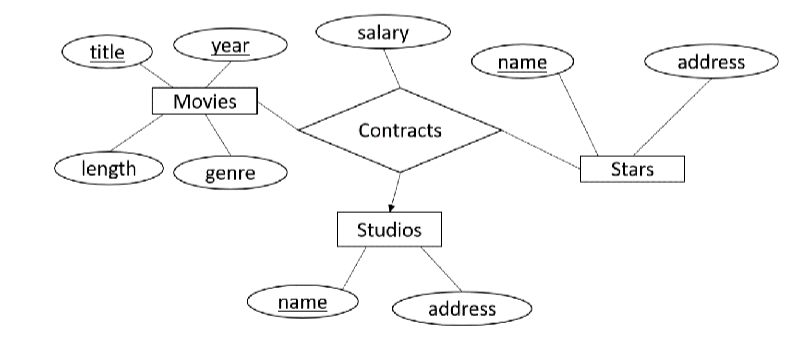
\includegraphics[scale = 0.8]{myndir/mynd1.png}
\end{center}

\vspace{1cm}

\section{15.}
Skrifið heilt Java forrit sem notar JDBC til að tengjast SQLite
gagnagrunni í skránni movies.db. Sá gagnagrunnur skal vera
kvikmyndagagnagrunnur eins og skilgreint er fremst í prófinu..
Forritið skal skrifa heildarlengd allra skráðra kvikmynda án þess að
nota hópun (GROUP BY).











\end{document}